%Version 3.1 December 2024
% See section 11 of the User Manual for version history
%
%%%%%%%%%%%%%%%%%%%%%%%%%%%%%%%%%%%%%%%%%%%%%%%%%%%%%%%%%%%%%%%%%%%%%%
%%                                                                 %%
%% Please do not use \input{...} to include other tex files.       %%
%% Submit your LaTeX manuscript as one .tex document.              %%
%%                                                                 %%
%% All additional figures and files should be attached             %%
%% separately and not embedded in the \TeX\ document itself.       %%

 
%%\documentclass[pdflatex,sn-nature]{sn-jnl}% Style for submissions to Nature Portfolio journals
%%\documentclass[pdflatex,sn-basic]{sn-jnl}% Basic Springer Nature Reference Style/Chemistry Reference Style
\documentclass[pdflatex,sn-mathphys-num]{sn-jnl}% Math and Physical Sciences Numbered Reference Style
\usepackage[utf8]{inputenc}
\usepackage[T1]{fontenc}
\usepackage{lmodern}
\usepackage{float}
\usepackage{tabularx}

%%\documentclass[pdflatex,sn-mathphys-ay]{sn-jnl}% Math and Physical Sciences Author Year Reference Style
%%\documentclass[pdflatex,sn-aps]{sn-jnl}% American Physical Society (APS) Reference Style
%%\documentclass[pdflatex,sn-vancouver-num]{sn-jnl}% Vancouver Numbered Reference Style
%%\documentclass[pdflatex,sn-vancouver-ay]{sn-jnl}% Vancouver Author Year Reference Style
%%\documentclass[pdflatex,sn-apa]{sn-jnl}% APA Reference Style
%%\documentclass[pdflatex,sn-chicago]{sn-jnl}% Chicago-based Humanities Reference Style

%%%% Standard Packages
%%<additional latex packages if required can be included here>

\usepackage{graphicx}%
\usepackage{multirow}%
\usepackage{amsmath,amssymb,amsfonts}%
\usepackage{amsthm}%
\usepackage{mathrsfs}%
\usepackage[title]{appendix}%
\usepackage{xcolor}%
\usepackage{textcomp}%
\usepackage{manyfoot}%
\usepackage{booktabs}%
\usepackage{algorithm}%
\usepackage{algorithmicx}%
\usepackage{algpseudocode}%
\usepackage{listings}%
\usepackage{placeins}
\usepackage{tabularray}%
\UseTblrLibrary{booktabs}%      
\usepackage{makecell}%  
\usepackage{placeins}%

\usepackage{tabularx}
\usepackage{array}
\usepackage{lipsum}
%%%%



%% as per the requirement new theorem styles can be included as shown below
\theoremstyle{thmstyleone}%
\newtheorem{theorem}{Theorem}%  meant for continuous numbers
%%\newtheorem{theorem}{Theorem}[section]% meant for sectionwise numbers
%% optional argument [theorem] produces theorem numbering sequence instead of independent numbers for Proposition
\newtheorem{proposition}[theorem]{Proposition}% 
%%\newtheorem{proposition}{Proposition}% to get separate numbers for theorem and proposition etc.

\theoremstyle{thmstyletwo}%
\newtheorem{example}{Example}%
\newtheorem{remark}{Remark}%

\theoremstyle{thmstylethree}%
\newtheorem{definition}{Definition}%

\raggedbottom
%%\unnumbered% uncomment this for unnumbered level heads
\renewcommand{\arraystretch}{1.15}
\setlength{\tabcolsep}{6pt}

\begin{document}

\title[Article Title]{"El uso de la inteligencia artificial para mejorar la experiencia educativa e interactiva en los museos de historia."}

%%=============================================================%%
%% GivenName	-> \fnm{Joergen W.}
%% Particle	-> \spfx{van der} -> surname prefix
%% FamilyName	-> \sur{Ploeg}
%% Suffix	-> \sfx{IV}
%% \author*[1,2]{\fnm{Joergen W.} \spfx{van der} \sur{Ploeg} 
%%  \sfx{IV}}\email{iauthor@gmail.com}
%%=============================================================%%

\author*[1,2]{\fnm{Erick} \sur{Guerron}}\email{erickguerron@yahoo.com}

\author[2,3]{\fnm{Maria} \sur{Zapata}}\email{paty1970maria@gmail.com}
\equalcont{These authors contributed equally to this work.}



\affil*[1]{\orgname{Universidad Técnica de Ambato}, \orgaddress{\street{}, \city{Ambato}, \postcode{}, \state{Tungurahua}, \country{Ecuador}}}


\abstract{The abstract serves both as a general introduction to the topic and as a brief, non-technical summary of the main results and their implications. Authors are advised to check the author instructions for the journal they are submitting to for word limits and if structural elements like subheadings, citations, or equations are permitted.}

\paragraph{Preguntas de Investigación} 
¿De qué manera la implementación de tecnologías de inteligencia artificial haría más interactiva la experiencia de los visitantes en los museos de historia?\newline
¿Qué beneficios educativos, culturales y tecnológicos aporta la implementación de inteligencia artificial en museos de historia?\newline
¿Qué ejemplos de aplicación de inteligencia artificial en galerías de arte han mostrado mejorar la experiencia del visitante?\newline
¿Cuál sería la influencia de la inteligencia artificial en la preservación y difusión del patrimonio cultural en comparación con métodos convencionales?\newline
¿Qué riesgos culturales o éticos podrían surgir de usar inteligencia artificial como herramienta para interpretar eventos históricos?\newline
¿Puede la inteligencia artificial reemplazar al guía humano en los museos históricos o deberíamos considerarla únicamente como un apoyo adicional?\newline


%%================================%%
%% Sample for structured abstract %%
%%================================%%

% \abstract{\textbf{Purpose:} The abstract serves both as a general introduction to the topic and as a brief, non-technical summary of the main results and their implications. The abstract must not include subheadings (unless expressly permitted in the journal's Instructions to Authors), equations or citations. As a guide the abstract should not exceed 200 words. Most journals do not set a hard limit however authors are advised to check the author instructions for the journal they are submitting to.
% 
% \textbf{Methods:} The abstract serves both as a general introduction to the topic and as a brief, non-technical summary of the main results and their implications. The abstract must not include subheadings (unless expressly permitted in the journal's Instructions to Authors), equations or citations. As a guide the abstract should not exceed 200 words. Most journals do not set a hard limit however authors are advised to check the author instructions for the journal they are submitting to.
% 
% \textbf{Results:} The abstract serves both as a general introduction to the topic and as a brief, non-technical summary of the main results and their implications. The abstract must not include subheadings (unless expressly permitted in the journal's Instructions to Authors), equations or citations. As a guide the abstract should not exceed 200 words. Most journals do not set a hard limit however authors are advised to check the author instructions for the journal they are submitting to.
% 
% \textbf{Conclusion:} The abstract serves both as a general introduction to the topic and as a brief, non-technical summary of the main results and their implications. The abstract must not include subheadings (unless expressly permitted in the journal's Instructions to Authors), equations or citations. As a guide the abstract should not exceed 200 words. Most journals do not set a hard limit however authors are advised to check the author instructions for the journal they are submitting to.}

\keywords{GenAI, Interactive Museums, Chatbots, Virtual Agent}

%%\pacs[JEL Classification]{D8, H51}

%%\pacs[MSC Classification]{35A01, 65L10, 65L12, 65L20, 65L70}

\maketitle

\section{Objetivos}
\subsection{Objetivo general}
\begin{enumerate}
    \item Analizar cómo la inteligencia artificial afecta a los museos dedicados a la historia.
\end{enumerate}

\subsection{Objetivos específicos}
\begin{enumerate}
    \item Examinar cómo la implementación de tecnologías de inteligencia artificial puede enriquecer la vivencia de los visitantes en los museos de historia.
    \item Identificar las ventajas educativas, culturales y tecnológicas que trae consigo la utilización de la inteligencia artificial en los entornos museísticos.
    \item Investigar casos concretos de la implementación de inteligencia artificial en museos y galerías, analizando su efecto en la experiencia del visitante y en la preservación del patrimonio cultural.
\end{enumerate}
  

\section{Introducción}\label{sec1}
\subsection{Descripción del problema}
Durante años los museos han cumplido con un papel central dentro de la interacción social con la cultura, ha sido una forma de aprender mediante experiencias sensibles así como son parte de los procesos relevantes para la preservación, reparación y difusión del patrimonio histórico y cultural. No obstante tras la pandemia y el auge de las tecnologías el número de visitantes que se acerca a estos espacios se ha reducido en base a que los mismos demandan experiencias que los conecten realmente con las exhibiciones, mediante una experiencia interactiva y personalizada que los lleve no solo a conocer sino a reflexionar y los transporte a la época de los hechos históricos descritos dentro de la exhibición estática de los objetos.

De este modo, se conoce que en diversos países se han encontrado soluciones tecnológicas  que buscaban modernizar la experiencia museística, un ejemplo claro se da con la creación de chatbots integrados en museos que permiten a los usuarios encontrar información, conocimiento y disfrute de experiencias, mediante una comparativa directa con la experiencia de usuario dentro de un aplicativo móvil de tours guiados, que en gran parte de esta época ha sido solución parcial a la diferencia tecnológica de espacios como museos. Esto describe  como mediante el uso de inteligencia artificial se puede mejorar la conexión con las temáticas presentadas dentro de los museos mediante la IA Generativa.\cite{Wang2025}

Dentro del mismo artículo se presenta que dentro de un aplicativo con Inteligencia Artificial Generativa integrada se reconocían los trabajos artísticos que el usuario estaba visualizando y después de esta recolección de datos se generaba información tanto visual como auditiva,\cite{Wang2025} lo cual demuestra que el uso de IA, de forma parcial, también permite a los usuarios con limitaciones de accesibilidad disfrutar de representaciones artísticas, del mismo modo el aplicativo generaba respuestas comunes mediante el manejo de una base de datos de los usuarios del aplicativo, demostrando mediante pruebas realizadas dentro del museo nacional del arte que la gente aprende más y disfruta más de la experiencia museística si interactúa con el agente conversacional que con un tour digital.

Del mismo modo otro proyecto presenta como los chatbots integrados a exhibiciones artísticas mejoran la conexión con el usuario, dicho proyecto, titulado “Enhancing Visitor Engagement in Interactive Art Exhibitions with Visual-Enhanced Conversational Agents” se enfocó en la construcción de un aplicativo dentro de museos de arte donde un agente conversacional multimodal que tenía percepción visual integrada interactuaba con los visitantes para alinear las interpretaciones artísticas de los mismo y fomentar la conexión con las representaciones artísticas. \cite{Ho2025} Mediante la participación de 36 individuos, este sistema mejoro el compromiso dentro del proceso de aprendizaje y análisis de los participantes así como genero conversaciones mas ricas entre el agente y los usuarios, De modo que dentro de este proceso evidencio que la integración de agentes conversacionales mejoraba la interacción cultural entre los usuarios y las obras.

Ambos contextos anteriores nos lleva a pensar que solo dentro del área del arte se puede aplicar estas soluciones, lo cual se ve reforzado dentro de una investigación más profunda, dentro del área del arte conectada con el conocimiento marítimo-biológico se presenta como una solución Mariscope, dentro de su artículo de creación “GenAI-Supported Creative Learning in Digital Museum Education: A Case Study of Maritime Art Painting Creation”, se presenta al aplicativo de IA generativa dentro de los contextos educativos con orientación a la creación de pinturas marítimas. Sus autores, Lin y Hu, reconocen mediante la investigación como las herramientas de Inteligencia Artificial generativa facilitan los procesos de aprendizaje al permitir al usuario interactuar con aspectos visuales, estéticos y conceptuales descritos por el arte marítimo donde mas que suplirla se busca fomentar su creatividad y comprensión artística con una experimentación guiada.\cite{Lin2025} 

Ademas en dicho estudio se aporta evidencia central de que la IA generativa no debe estar limitada solo a la generación de contenido visual sino que enriquece procesos de aprendizaje que de otras formas podrían ser imposibles como lo es la exploración marina, así también beneficia al proceso de aprendizaje musaico digital, de forma que se busca no solo un impacto visual del arte sino uno emocional mediante el análisis de experimentación de las obras.\cite{Lin2025}

Sin embargo, como varios artículos analizados para la construcción de la idea presentada se limita a un campo especifico de estudio dentro del ámbito artístico, lo cual deja mucho terreno por descubrir en museos relacionados con la historia o con otras colecciones culturales. Analizar solo el campo artístico limita de forma importante al uso de la IA generativa, ya que contextos como el histórico ofrecen oportunidades únicas que conectarían a los visitantes del museo con la época donde de la que proviene el objeto expuesto, permitiendo el análisis de experiencias que no se pueden experimentar directamente pero entendiéndolas dan una mayor conexión entre la historia y el individuo. El uso de IA generativa dentro de este espacio no solo personalizaría los recorridos, la manera en que las exhibiciones se colocan o enriquecer procesos narrativos sino que compromete al usuario a una apropiación del conocimiento histórico donde existe una interacción con el pasado de manera dinámica con contextualización que permita construir preguntas más profundas que lleven a más procesos de aprendizaje.

\subsection{Preguntas de Investigación}
\begin{enumerate}
    \item ¿De qué manera la implementación de tecnologías de inteligencia artificial haría más interactiva la experiencia de los visitantes en los museos de historia? 

    \item ¿Qué beneficios educativos, culturales y tecnológicos aporta la implementación de inteligencia artificial en museos de historia? 

    \item ¿Qué ejemplos de aplicación de inteligencia artificial en galerías de arte han mostrado mejorar la experiencia del visitante? 

    \item ¿Cuál sería la influencia de la inteligencia artificial en la preservación y difusión del patrimonio cultural en comparación con métodos convencionales? 

    \item ¿Qué riesgos culturales o éticos podrían surgir de usar inteligencia artificial como herramienta para interpretar eventos históricos? 

    \item ¿Puede la inteligencia artificial reemplazar al guía humano en los museos históricos o deberíamos considerarla únicamente como un apoyo adicional? 
\end{enumerate}

\subsection{Justificación}
Desde tiempos inmemoriales la humanidad ha buscado preservar su historia mediante la creación y protección de artículos ancestrales, dichos artículos forman parte de las vivencias de las culturas que formaron los modos de vida actuales ya que cimentaron las bases de nuestra sociedad. De aquí nace la importancia de espacios donde estos objetos sean preservados como lo son los museos.

Un lugar altamente importante dentro del aprendizaje no solo cultural ni artístico sino también histórico corresponde al museo. Que desde su concepción busca facilitar el acceso a la historia mediante la presentación de aquellos objetos pero evitando que estos sufran las inclemencias del tiempo o faltas a las normas por pensamientos poco críticos que terminan en actos de vandalismo. De modo que los museos permiten mediante este proceso de protección que futuras generaciones tengan el mismo acceso a la historia que las actuales para que conecten con experiencias pasadas, comprendan contextos históricos y valoren la diversidad de culturas dentro de épocas distintas a las de su visita.

Dentro de una era totalmente industrializada, el uso de la tecnología se ha integrado a espacios como los museos, de modo que dentro de los estudios analizados uno de los autores [Chen, Duan]la tecnología es utilizada para mejorar la experiencia dentro de estos espacios, como el uso de realidad virtual dentro de los espacios pedagógicos permite a los estudiantes conectar mediante la interacción directa con el contenido y facilita el trabajo en colaboración,\cite{Chen2021}de modo que la integración de estos espacios en museos mejora la conexión y la generación de experiencias del visitante con mayor tolerancia en usuarios con capacidades especiales, de modo que el beneficio se extiende porque se basa en la recreación exacta dentro del aprendizaje.

De modo que el punto anteriormente expuesto refuerza que existe un proceso de transición entre el desarrollo tecnológico dentro de estos espacios, dentro del articulo Technology and museum visitor experiences: a four-stage model of Evolution, que pertenece los autores [Lu, Moyle, Red, Yang,Liu] se muestra un proceso de mapeo de la evolución mediante clasificación de las épocas y las tecnologías, donde se reconoce que existe una transición desde el uso de herramientas informativas como guías, audio guías o mapas hacia soluciones inteligentes soportadas mediante IOT o análisis de datos, y es dentro de este articulo se destaca que los procesos de escalabilidad hacia mejores soluciones de UX en instituciones donde esto es posible mejoran la experiencia de los usuarios con conexión más significativa.\cite{Lu2023}

Pero este contexto no solo se limita hacia el uso de realidad virtual o IOT dentro del mejorar experiencias en museos sino que en otros artículos como el [Siri] donde se demuestra mediante una revisión de literatura en Scopus como la IA cada vez es mas usada dentro de museos para generar experiencias personales, procesos de preservación digital y gestión de exhibiciones, sin negarse a los riesgos de la misma como el sesgo, la ética de trabajo en IA, los limites de transparencia en los datos personales donde se reconoce que dando el espacio a la IA de forma responsable permite que no solo mejore la experiencia del museo pero también lo compromete con una inclusividad donde se salvaguarda los roles de progreso hacia el conocimiento cultura y desarrollo de educación.\cite{Siri20242038}

Así mismo ExhibitXplorer demostró ser una solución para la entrega de contenido personalizado según ubicación del visitante con reconocimiento de sus preferencias de forma explícita e implícita mediante la georeferenciación así como la IA, dicho artículo demostró que mediante microservicios con notificaciones y segmentación del visitante así como su información se generó un modelo de lenguaje para generación automática de texto que brinda actualizaciones donde mediante las pruebas se mostró una gran aceptación de los visitantes, aunque el proceso genero latencia, así como dificultades en la seguridad de que el contenido sea correcto y culturalmente apropiado.\cite{ijgi12100434}

Esto demuestra que el uso de IA mejora la experiencia de aprendizaje, ademas de ser aceptada por el usuario ya que al tener una experiencia personalizada no solo se gana que el usuario conecte con la temática de la exhibición sino que la misma permite que el usuario marque su propia curva de aprendizaje en función de la inferencia del sistema hacia el mismo.

Desde un punto similar, el autor [Liu] toma el avance de la inteligencia artificial que desde este punto ha incrementado su uso dentro de museos, en su articulo realiza un analisis literario donde se examina las aplicaciones que tienen sistemas integrados con IA dentro de museos, asi como la identificación de los principales retos en su construcción, adaptación y manejo asi como las soluciones dadas por sus desarrolladores con un exploración de las tendencias futuras. Dentro de este articulo se revela que el uso de IA mejora de forma significativa dando experiencias personalizadas, inmersivas y con mayor servicio hacia la accesibilidad.\cite{Iodice2025AI}

De igual modo dentro del manejo de la operabilidad la IA demuestra notablemente ventajas en control de costos y promueve la optimización de eficiencia, de forma efectiva mejora la reutilización de los recursos. Igualmente la AI promueve la integración de cultura así como de tecnología, punto que permite reconocer que el uso de IA promueve mas ventajas para los usuarios ya que no solo los conecta con la experiencia sino que potencia sus capacidades en función de una experimentación del hecho, donde la herencia cultural se fortalece y el proceso educativo se vuelve más activo.

Estudios más profundos donde se ha llevado fuera del contexto analítico el uso de Inteligencia Artificial demuestran que es una fuerte solución a las técnicas anteriormente empleadas para el recorrido de museos, no solo porque la IA genera un porcentaje mayor de confianza hacia el usuario, donde sin importar el nivel de pregunta que el mismo genere la IA resolverá su duda, sino que no lo limita al conocimiento del guía de modo que en exhibiciones de gran interés para el visitante esta permite un análisis más profundo.

Uno de ellos corresponde al presentado por [Tripathi, Munshi], mismo que estudia las experiencias interactivas dentro del arte como las experiencias presentadas por The Van Gogh Museum y el Cooper Hewitt Smithsonian Design Museum, tomando en cuenta que los mencionados tiene sistemas inteligentes con manejo de la información del visitante para alterar la disposición de los cuadros, la iluminación, donde se genere navegaciones con activación de voz así como transiciones entre exhibiciones con tiempo real, los museos mencionados anteriormente son tomados como caso de uso de este articulo donde se toma en cuenta que la AI puede generar eficiencia operacional  mediante la generación de una experiencia personalizada donde se preserva la privacidad de visitante mediante su consentimiento, presentando una solución para una experiencia interactiva donde se mejora la accesibilidad del publico así como la experiencia del usuario y el manejo energético.\cite{Tripathi2025HumanCentered}

No obstante, aunque todas las investigaciones anteriores demuestran que la IA es una herramienta fuerte para el desarrollo de experiencias más significativas dentro de museos, muchas de ellas corresponden a ideas o contextos especificos, como el arte, dejando un vacío dentro del espacio de los museos históricos. Es de este modo que en este proyecto, se propone explorar como la inteligencia artificial generativa puede aplicarse en el ámbito histórico con la finalidad de mejorar la interacción de los visitantes, personalizando sus recorridos en función del análisis de sus características, facilitando la comprensión de contextos pasados mediante una experimentación realista de manera más efectiva.

\section{Metodología}\label{sec11}

La metodología seleccionada para este estudio es de carácter exploratorio y cualitativo, ya que el mismo busca analizar de manera preliminar el potencial del uso de la inteligencia artificial generativa dentro de museos históricos, un campo que ha sido poco desarrollado dentro de la literatura. Para este enfoque se plantea tres fases principales dentro de su ejecución.

\begin{figure}[h] % h = here (aquí)
    \centering
    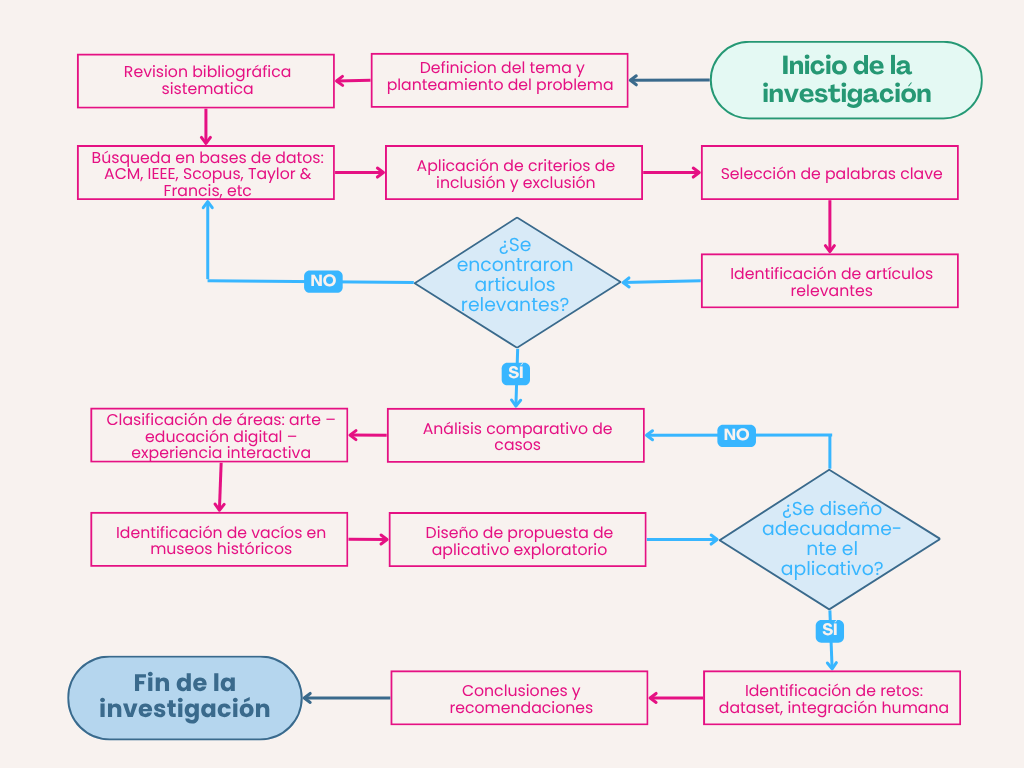
\includegraphics[width=0.7\textwidth]{images/Grafica Diagrama de Flujo Profesional Beige.png}
    \caption{\centering Diagrama de flujo de la metodología.}
    \label{fig:metodologia}
\end{figure}

En la fase inicial, se realiza una revisión bibliografía sistemática de investigaciones recientes que se encuentren relacionadas con el uso de la Inteligencia Artificial generativa dentro de espacios culturales en entornos como museos y educativos. El proceso de investigación contempla la búsqueda de artículos dentro de bases de datos académicas como ACM Digital Library, IEEE Xplore, Scopus, Taylor and Francis, entre otras mediante la aplicación de criteros de inclusión como: publicaciones de los últimos siete años, uso de IA generativa, uso de agentes conversacionales o chatbots y estudios en el contexto de museos, espacios del arte y educación.

Un ejemplo claro de la técnica empleada para la búsqueda mediante el uso de keywords corresponde al acceso que se dio del articulo Smart Museums, Smarter Experiences: Exploring the Impact of GenAI Usability on Digital Heritage Enjoyment, dicho artículo se encontró mediante el uso de la combinación de las palabras claves “GenAI” y “Museums”, estas dos palabras fueron las principales a tomarse en cuenta dentro del analisis de los títulos de los artículos a analizar dentro de los distintos sitios. Dentro de las palabras seleccionadas para las búsquedas se encuentan aparte de las dos mencionadas anteriormente “Digital Education”, “Visitor engagement”, “History Museums”, “AI”, “Conversational Agent”, que se establecen como guia para la investigación.

Dentro de la segunda fase, se propone un análisis comparativo de los casos identificados con la finalidad de identificar las áreas donde la AI presenta mayor visibilidad (arte, educación digital, experiencia interactiva) de modo que se refuerce la evidencia de la brecha en el ámbito de museos histórico, que demostraría si la elección temática es la correcta dentro del campo de análisis.

Finalmente dentro de la última fase del proyecto, se desarrollara una propuesta inicial de aplicativo, que describe de forma real como la IA generativa puede implementarse dentro de los museos históricos del país con la generación de itinerarios en función de las preferencias del usuario, manejo mediante chat de las preguntas del usuario con respecto a una exhibición en concreto, y que retos propondría el uso de una solución de este estilo a gran escala, como correspondería la realización de un data set para la construcción de los agentes conversacionales y como este proceso integraría al personal humano que maneja estos espacios.

Es por ello que dentro de la fase final del proyecto, la propuesta contemplara los siguientes aspectos:

\begin{enumerate}
    \item Personalización de itinerarios mediante el análisis de preferencias de los usuarios con recorridos adaptados mediante la priorización de objetos y exposiciones que se alinean con los intereses de dicho usuario.
    \item Interactividad mejorada mediante la relación entre usuarios y agentes virtuales que respondan preguntas, cuenten historias sobre objetos, proporcionen información contextual extra o representen a la personalidad sobre la que se engloba la exposición, mejorando el aprendizaje contextualizado, es en este punto que se analizara si manejar un sistema de comandos por voz, un agente de chat o realidad aumentada con IA de fondo.
    \item Reorganización de espacios conceptuales mediante sugerencias a los organizadores de las exhibiciones para facilitar experiencias inmersivas mediante recorridos temáticos o agrupación de piezas.
    \item Mecanismos de evaluación para retroalimentación básica del sistema en función de la opinión del usuario que permita mejorar de forma iterativa la experiencia y ajustar el itinerario en futuras implementaciones, mediante una encuesta corta de satisfacción al final de cada visita.
\end{enumerate}

\subsection{Limitaciones de la Investigación}
\begin{enumerate}
    \item \textbf{Característica exploratorio y no generalizada. } \\
    El presente estudio es de carácter exploratorio y cualitativo, por lo que su intención principal es abrir camino en un tema poco trabajado, en lugar de brindar conclusiones universales. Los resultados obtenidos se deben tomar como una orientación futura para investigaciones posteriores y no como respuestas definitivas. 
    \item \textbf{Dependencia de artículos ya publicados. } \\
    Al apoyarse de gran manera en las revisiones de estudios previos los hallazgos dependerán de trabajos de otros investigadores publicados en bases de datos académicas. 
    \item \textbf{Limitantes en la búsqueda de información relevenate. }\\
    El presente estudio es de carácter exploratorio y cualitativo, por lo que su intención principal es abrir camino en un tema poco trabajado, en lugar de brindar conclusiones universales. Los resultados obtenidos se deben tomar como una orientación futura para investigaciones posteriores y no como respuestas definitivas.
    \item \textbf{Propuesta sin validación en la practica.  }\\
    La solución propuesta para la implementación de la IA en museos históricos es, por ahora, una propuesta conceptual. No se va a implementar en un entorno real, por lo que no se pueden sacar datos reales sobre su eficacia y reacción de los visitantes, ademas de las dificultados técnicas que podrían surgir y los ajustes necesarios en la practica. 
    \item \textbf{Enfoque centralizado en contexto especifico. }\\
    El análisis se centraliza principalmente para la aplicación en museos históricos de nuestro país. Esto limita la aplicabilidad de los resultados en otros contextos, donde los museos puedan presentar diferentes recursos, públicos y niveles de digitalización. 
    \item \textbf{Aspectos tecnológicos y éticos aun por profundizar. }\\
    Aunque el presente estudio menciona algunos retos como los sesgos producidos por la dependencia a la IA, la necesidad de infraestructura o el papel que cumple el personal humano frente a los agentes virtuales, estos temas no se profundizan. Son aspectos complejos que requieren de estudios as detallados y especializados en un contexto futuro. 
\end{enumerate}

\section{Marco teórico}
Este marco teórico describe el uso de la inteligencia artificial (IA) para personalizar y mejorar la experiencia educativa e interactiva en los espacios de narración de historias. La revisión se organiza en cuatro secciones: museos y educación, inteligencia artificial en entornos culturales, inteligencia artificial generativa y experiencias personalizadas, así como la brecha en los museos históricos.

\subsection{Museos y educación}   
Los museos han desempeñado históricamente un papel fundamental en la conservación del patrimonio cultural y en la transmisión del conocimiento. Además de su función expositiva, estos espacios se presentan como entornos de aprendizaje no formal, donde los visitantes pueden acceder a experiencias educativas que integran la observación, la interpretación y la reflexión crítica. La digitalización ha ampliado esta misión pedagógica al incluir audioguías, plataformas digitales y aplicaciones de realidad aumentada.
En este contexto, el Museo Nacional Thyssen-Bornemisza ha integrado de manera sistemática tecnologías digitales en las áreas de comunicación, educación y conservación. Entre sus proyectos destacados se encuentran EducaThyssen. org y Second Canvas Thyssen, los cuales fortalecen la dimensión educativa del museo a través de experiencias interactivas \cite{espadas2025}.

\subsection{Inteligencia Artificial en Entornos Culturales}
La incorporación de la inteligencia artificial en los entornos culturales ha transformado tanto la gestión institucional como la experiencia del visitante. Según Espadas (2025), se documenta cómo la digitalización ha permitido optimizar los procesos museísticos y ampliar las estrategias educativas. De forma complementaria, un estudio multinacional llevado a cabo con 110 estudiantes universitarios de seis países revela que el 87,29\% de los participantes opina que la inteligencia artificial (IA) puede mejorar la accesibilidad de las colecciones. Por otro lado, aspectos como la personalización (27,3\%) y la motivación (25,4\%) son considerados fundamentales para enriquecer la experiencia educativa \cite{suicmez2025}. Estos hallazgos demuestran que la inteligencia artificial no solo mejora la gestión interna, sino que también promueve la inclusión y el aprendizaje participativo.

\subsection{Inteligencia Artificial Generativa y Experiencias Personalizadas}
La inteligencia artificial generativa ofrece nuevas oportunidades para la creación de experiencias museísticas personalizadas. Herramientas como chatbots conversacionales, sistemas de reconocimiento visual y motores de recomendación permiten diseñar itinerarios personalizados para cada visitante. El "ReInHerit Toolkit", presentado por Mazzanti y colaboradores. El trabajo de Mazzanti (2025) integra chatbots y análisis visual inteligente con el objetivo de fomentar el aprendizaje interactivo. De manera similar, Ivanov \cite{ivanov2024advanced} propone un sistema de insignias inteligentes que utiliza tecnología BLE, lo que permite la personalización dinámica de contenidos según la ubicación y los intereses del visitante.
Sin embargo, la dependencia excesiva de los sistemas de diálogo basados en inteligencia artificial puede tener efectos negativos. Zhai y Tang \cite{zhai2024effects} advierten que el uso acrítico de estas herramientas puede disminuir las capacidades de pensamiento crítico y analítico. Baker y Hawn \cite{Baker2022Algorithmic} también destacan que los sesgos algorítmicos en los sistemas educativos pueden poner en riesgo la equidad y la transparencia. Por lo tanto, es necesario establecer marcos éticos robustos en el diseño de experiencias museísticas.

\subsection{La Brecha en los Museos Históricos}
A pesar de los avances en los museos de arte y ciencia, la aplicación de la inteligencia artificial en los museos históricos sigue siendo limitada. Derda y Predescu \cite{Derda2025HumanCentric} enfatizan la relevancia de adoptar un enfoque centrado en el ser humano (HC-AIM). En este contexto, la aceptación tecnológica por parte del personal de los museos y la preservación de la visión curatorial son factores esenciales para el éxito de estas iniciativas. En paralelo, Lei \cite{lei2025artificial} propone un modelo de optimización espacial basado en inteligencia artificial que mejora la fluidez del recorrido en un 18,1\%, reduce la congestión y aumenta la tasa de visitas a las exhibiciones en un 50\%. Este estudio demuestra que la disposición física también puede ser un recurso educativo.
Sin embargo, estas innovaciones se han centrado principalmente en la estética y la disposición espacial, mientras que la narrativa histórica necesita un tratamiento especializado. La contextualización temporal, la preservación de la memoria colectiva y el fomento de la reflexión crítica continúan siendo desafíos en la implementación de la inteligencia artificial en museos históricos. Esta brecha representa una oportunidad para futuras investigaciones centradas en la educación patrimonial y en el fortalecimiento de la interacción entre los visitantes y la historia.

\subsection{Síntesis}
En resumen, la literatura revisada sugiere que la inteligencia artificial puede mejorar la accesibilidad, la personalización y la motivación en entornos museísticos, teniendo un potencial considerable para crear experiencias educativas más inclusivas e interactivas. No obstante, persisten riesgos asociados a la dependencia tecnológica y a los sesgos algorítmicos, así como una brecha en la implementación de estas tecnologías en museos históricos. El desafío actual consiste en adaptar las innovaciones de la inteligencia artificial generativa a la narrativa histórica, asegurando un equilibrio entre la innovación tecnológica, la gobernanza ética y la preservación cultural.

\FloatBarrier
\begin{table}[!ht]
  \centering
  \caption{Artículos adicionales y sus aportes a la investigación}
  \label{tab:articulos-aportes}
  \begin{tblr}{
    colspec = {@{} l l X X @{}}, % l,l y dos columnas flexibles
    row{1} = {font=\bfseries},   % encabezado en negrita
    rowsep = 2pt
  }
    \toprule
    Referencia & Tipo / Enfoque & Aporte principal & Relevancia para este estudio \\
    \midrule
    \cite{espadas2025} & Estudio de caso institucional &
    Integración sistemática de tecnología en comunicación, educación (EducaThyssen; RA con Second Canvas), exposiciones y restauración; marco de transformación digital. &
    Marco de referencia práctico para estrategias de transformación digital en museos de historia/arte. \\
    \cite{suicmez2025} & Estudio cualitativo (n=110, 6 países) &
    Evidencia de que la IA mejora accesibilidad (87.29\%), personalización (27.3\%) y motivación (25.4\%). &
    Soporte empírico para metas educativas e interactivas basadas en IA en museos históricos. \\
    \cite{murphy2022red} & Guía profesional / toolkit &
    Casos (Prado, National Gallery, Met), evaluación de capacidades, ética y mapeo de stakeholders. &
    Hoja de ruta operativa y ética para implementar IA con gobernanza responsable. \\
    \cite{mazzanti2025reshaping} & Toolkit / demostradores &
    Chatbots, reconocimiento de poses y análisis visual para experiencias interactivas personalizadas. &
    Catálogo de soluciones replicables para diseño de experiencias educativas con IA. \\
    \cite{ivanov2024advanced} & Propuesta técnica aplicada &
    Badges BLE + perfilado explícito/implícito; localización y grupos por proximidad; contenido con IA (ChatGPT). &
    Arquitectura concreta para personalización in situ y segmentación dinámica de visitantes. \\
    \cite{lei2025artificial} & Optimización con IA (RL, CV, afectiva) &
    Mejora de fluidez espacial (+18.1\%), menos congestión y +50\% en visitas; adaptación por emociones. &
    Evidencia de impacto de IA en diseño espacial e interactividad de recorridos. \\
    \cite{Derda2025HumanCentric} & Modelo de gobernanza (HC-AIM) &
    Enfoque centrado en el humano; aceptación tecnológica del personal; co-creación de valor. &
    Asegura alineación ética/curatorial; clave para adopción y sostenibilidad del sistema. \\
    \cite{zhai2024effects} & Revisión sistemática (14 estudios) &
    Riesgos por sobredependencia de diálogo-IA: menor decisión (–27.7\%), pensamiento crítico y analítico. &
    Advierte sobre marcos de uso que preserven habilidades cognitivas en experiencias educativas. \\
    \cite{Baker2022Algorithmic} & Revisión / marco conceptual &
    Sesgos algorítmicos y equidad en educación; transparencia y mitigación de bias. &
    Fundamenta métricas de equidad/transparencia en sistemas IA para narrativa histórica justa. \\
    \bottomrule
  \end{tblr}

  \vspace{2pt}
  {\footnotesize\textit{Nota:} RA = Realidad Aumentada; BLE = Bluetooth Low Energy; RL = Aprendizaje por refuerzo; 
  CV = Visión por computadora; HC-AIM = Human-Centred AI in Museums.\par}
\end{table}
\FloatBarrier



\section{Resultados}\label{sec2}

Dado el exhaustivo análisis presentado dentro del marco teórico de este articulo así como tras el reconocimiento de los recientes avances de la aplicación de la inteligencia artificial dentro de los entornos museísticos así como de la brecha existente en la aplicación de esta herramienta dentro del ámbito histórico, se plantea a continuación una propuesta de solución que se encuentra orientada a aprovechar todas las ventajas de las capacidades de la IA generativa dentro del espacio de aprendizaje propuesto por los museos.

\subsection{Propuesta de solución}

El objetivo de esta solución es enriquecer la experiencia de los visitantes mediante la generación de recorridos personalizados, la fomentación de la interactividad en las exhibiciones mediante un proceso de aprendizaje conversacional y brindar a los gestores de los museos herramientas que faciliten la toma de decisiones para la gestión de estos espacios así como de los contenidos presentados mediante el acercamiento de la información sobre el nivel de satisfacción de los visitantes.

Esta interactividad mencionada dentro de las visitas de los usuarios busca ser promovida mediante el proceso de aprendizaje conversacional, inspirado en la mayéutica socrática, en el cual el usuario no solo recibe la información de forma pasiva, proceso que puede sobre estimularlo o confundirlo, si no que construye su propio conocimiento mediante una serie de preguntas y respuestas dentro del dialogo con el agente virtual de la exhibición. De modo que se le otorga al usuario la opción de guiar la conversación según sus intereses y nivel de curiosidad, favoreciendo la experiencia reflexiva y personalizada.
. 
La propuesta parte del diseño de un aplicativo basado en una arquitectura de capas tipo Onion, que se encarga de separar responsabilidades a cada una de las capas del aplicativo. Se propone que para un proyecto de la escala del planteado dentro de este artículo se utilice por lo menos una capa para interfaz, una para la lógica de dominio, una para exposición de servicios, una para servicios y una de persistencia. Del mismo modo se considera que esta arquitectura facilitara la verificación y gobernanza de la información. 

El sistema propuesto busca integrar una capa de entrada para la captura de las preferencias del usuario, donde se maneje de forma íntegra todos los datos, este proceso se realizara tanto dentro de la entrada al museo como durante su exploración, por lo cual dentro de su recorrido el usuario visualizara las dos posibles salas a las que puede ir después de recorrer una exhibición, posterior a ello un proceso de análisis se realizara dentro de las salas con una detección de presencia en sala que detectara la exhibición en la que el usuario se encuentra.

Una capa de dominio que se encargara de orquestar recomendaciones y las agentes conversaciones se encuentra después, esta viene de la mano con el dato de detección anteriormente mencionado ya que los agentes conversaciones se personalizaran en función de las exhibiciones existentes, una capa de datos manejara la centralización de las fuentes validad y los dataset curados por los guías pertenecientes al museo que se encargaran de brindar información a los agentes virtuales.

Dentro de la capa de infra servicios se encontraran los modelos LLM así como los sistemas de embeddings y las bases matriciales de datos así como las APIs encargadas de nutrir información a las capas superiores basadas en técnicas de recuperación y generación (RAG) Siendo esta solución una prueba de la priorización de la validación humana del contenido presentado, ya que los mismos guías verificaran los datos presentados por los agentes virtuales, así como un ciclo de mejora continua mediante la retroalimentación de los usuarios y los empleados del museos.

La recolección del conocimiento de los agentes se realiza principalmente mediante los dataset especializados que se recopilaran en el momento en el que se planee una exhibición dentro de este sistema, estos dataset pasaran por un proceso de validación y verificación por el personal del museo. Cada exhibición contara con un dataset especifico disponible donde se encuentren descripciones, preguntas comunes, referencias bibliográficas y anotaciones, las cuales serán versionadas y sometidas a verificación humana antes de ser indexadas.

Dentro del proceso de verificación de datos en la capa de modelos con IA generativa se propone contar con filtros de seguridad así como políticas de contenido y post-procesado para evitar la mayor falla de la IA generativa que corresponde a los procesos de alucinaciones, estos filtros como se mencionó anteriormente serán llevados en proceso de validación humana, donde un empleado del museo sube información o la edita, un experto la revisa, la marca como verificada, se da una última revisión al dato alterado o agregado dentro del dataset y se despliega dentro del entorno de referencia.

Se propone que dentro del LLM se utilice generación aumentada por recuperación o RAG ya que este mediante el uso de su combinación tanto mediante sistema tradicional de recuperación de información con uso de búsquedas y base de datos así como el uso de las capacidades del modelo generativo de lenguaje extenso de modo que la respuesta sea más precisa, actualizada y relevante en función de las necesidades conversacionales del agente dentro de la exhibición.

Una de las principales fortalezas del uso de generación aumentada de recuperación viene de sus potentes algoritmos de búsqueda que permiten el uso de consultas a datos externos, como páginas web, bases de conocimiento \cite{google2025rag} y dentro del modelo propuesto, el sistema de datos que será montado y actualizado en función de lo especificado por los guías de museo, la generación fundamentada que es el resultado de la recuperación y preprocesamiento dentro de los algoritmos de búsqueda permitirán que el agente conversacional no caiga en alucinaciones. Del mismo modo el usar RAG permite que el LLM se limite a sus datos previamente entrenados.

Pero esto nos pone nuevamente en un potencial problema, que pasa si un usuario hace una pregunta que se encuentra fuera de nuestra base, la solución propuesta a este predicamento radica en dos posturas, uno, que los guías resuelvan la duda en el momento en el que este usuario la haga, es decir se notifique al guía encargado de la falta de este dato, a lo que el contestara en ese momento y actualizara la base de datos; dos, si esto no es posible ya que no existe conocimiento técnico o histórico como respuesta de la pregunta del usuario entonces se mandara un mensaje de error que le notifique pero no saque al usuario de la experiencia inmersiva y se propondrá mayores investigaciones dentro de esta área, a fin de que en algún punto se pueda encontrar información para solventar esa duda.

De este modo el sistema no solo mejoraría la experiencia de los usuarios mediante la interacción directa con el contenido histórico basada en solución de preguntas y respuestas sino que también convertiría este aplicativo en una fuente de opciones para futuras investigaciones que nutran de información específica para el mejoramiento de la base de datos que la integran.

La exposición de los servicios de soporte para la escalabilidad del aplicativo estará dada por la capa de infraestructura con exposición de servicios. De modo que las APIs REST así como GraphQL permitirían la comunicación entre la interfaz del usuario, los agentes conversacionales y los sistemas de análisis, del mismo modo dentro de esta capa se llevara acabo procesos relacionados con la autentificación y encolado garantizara que exista seguridad y gestión eficiente entre las solicitudes.

Con un análisis mayor se tomara esta capa como soporte técnico para todas las funciones del aplicativo tenga un funcionamiento fluido, seguro y escalable. Dentro de su planteamiento se espera que esta capa sirva como puente entre la interfaz y los servicios internos de aplicativo de los cuales destaca el motor de recomendación de itinerarios y los agentes conversacionales. Ademas esta capa se encargara de permitir que la información del usuario, fluya hacia la capa de datos y regrese como parte del análisis de los procesos de esta capa de forma en que se garantice que las respuestas sean contextuales y actualizadas a tiempo real, haciendo que este sea un sistema de respuesta rápida.

Ademas la capa de exposición de servicios asegurar que cada visitante solo acceda a los servicios y agentes correspondientes a la exhibición en la que se encuentra de modo que trabajaría con los sensores a implementarse como medidores de ubicación para el usuario. Del mismo modo que puede incluir autentificación ligera basada en códigos QR alrededor de las exhibiciones que eviten que el usuario necesite contar con un usuario preestablecido antes de su visita, o una opción que puede ser mas costosa pero mejor implementada corresponde a la detección mediante proximidad con sensores, mismos que podrían ser parte de las exhibiciones de modo en que el sistema verifique en que exhibición el usuario se encuentra  antes de darle acceso al agente conversacional de modo que se asegure de que este se encuentre 
activo para su interacción con el usuario solo en su contexto especifico.

Mediante el uso de tecnologías tipo RabbitMQ,que corresponde a un middleware orientado a mensajes y un agente de mensajes de código abierto que actúa como intermediario dentro de comunicaciones asincrónicas entre aplicativos para facilitar enrutamiento, gestión de colas y entrega en sistemas distribuidos,o a su ves KAFKA puede manejar múltiples interacciones de forma simultánea dentro de la opción de interacción grupal para que se pueda tener un manejo de datos controlado en exhibiciones de alta afluencia de visitantes, de modo que el sistema sea escalable y adaptable a las condiciones del museo, donde existe una priorización de solicitudes así como manejo de colas de interacción donde se garantiza que cada agente responde de manera coherente sin provocar sobrecargas dentro del motor de recomendaciones para la construcción de los recorridos o los modelos de IA generativa.

Para que exista mayor facilidad dentro de la trazabilidad de cambios y actualizaciones de contenidos que será la mayor fortaleza del sistema, se propone un almacenamiento centralizado con sistemas tipo en S3 o equivalentes para guardar los dataset verificados de las exhibiciones, tener un sistema S3 permite que cada cambio sea guardado mediante un histórico, de forma en que si se comete un error este pueda ser revertido y controlado de forma automática. Tanto los logs de interacción de los visitantes así como las métricas de uso será utilizadas mediante este sistema ya que los sistemas S3 o Amazon Simple Storage Service  manejan un gestiona miento de objetos dentro de la nube con cubos con clave única.

Tomando la perspectiva de su creador, S3 es un servicio de almacenamiento de objetos con escalabilidad, disponibilidad de datos, búsqueda de la seguridad y rendimiento dentro de sistemas con gran cantidad de datos sin importar el uso de estos. AWS destaca que S3 permite un manejo ágil de la información dentro de aplicaciones nativas de nube así como en móvil, que sería la forma de trabajo dentro del aplicativo propuesto. Del mismo modo S3 tiene un optimización de costes así como dentro de la organización y análisis de los datos lo cual facilitaría los procesos de acceso dentro del aplicativo mejorando la respuesta entre las interacciones de las distintas capas del sistema.\cite{aws_s3}

Finalmente se espera que la capa de infraestructura y exposición de servicios sea la encargada de los servicios relacionados con BI, y que por esto tomando los logs así como las métricas entregadas por el aplicativo, genere dashboards para los gestores del museo. Con indicadores enfocados en las áreas más visitadas, los agentes más consultados, las preguntas más frecuentes, las preguntas donde no existió la suficiente información, los recorridos más comunes así como los patrones de interacción y los resultados estandarizados del nivel de satisfacción tras la visita. De forma en que se facilite la toma de decisiones sobre las áreas de inversión dentro del museo, las exhibiciones a reforzar y como mejorar la experiencia de usuarios.

De modo que dentro de la capa de infraestructura se espera lograr un soporte de coherencia, escalabilidad y seguridad dentro del aplicativo. Esta capa será el sello de confiabilidad de los agentes conversacionales. Se encargara de las actualizaciones en tiempo real de los itinerarios personalizados y de la gestión de los museos para la toma de decisiones más fundamentadas en la información valiosa de la experiencia de los visitantes. 

Dentro del aplicativo se contara también con un repositorio maestro o RBDMS relacional que se puede manejar tanto mediante el uso de PostgresSQL o a su vez mediante MySQL que se encuentre centralizado para el almacenamiento de datos estructurados sobre las posibles exhibiciones, los horarios de apertura del museo así como los accesos permitidos, los distintos roles de los usuarios donde se gestionaría los accesos tanto del visitante como de los guías y gestores de información para los LLM.

A parte del repositorio maestro de la información que manejaría la información relacionada con los visitantes y el personal se tendría colecciones de información verificada por los guías y gestores donde se tomaría en cuenta textos curatoriales, artículos académicos sobre las posibles temáticas, transcripciones de guías y catálogos existentes. Dentro de este punto se sugiere como aplicativo un data lake cimentado dentro de S3 organizado mediante carpetas que correspondan a la exhibición así como al tipo de medio, como se explicó dentro del apartado de la capa relacionada con los agentes conversacionales, los dataset a utilizarse pasarían por procesos de validación manual mediante interacción con historiadores y curadores antes de ser integrados dentro del sistema.

Para apoyar al proceso de recuperación semántica mediante el uso de RAG se propone del mismo modo un Vector DB con bases sugeridas como Pinecone, Weaviate o FAISS que se encarguen de los procesos de indexación de la información en forma de vectores para las consultas temáticas. A modo de ejemplo del proceso a realizarse se propone que un visitante pregunte ¿Qué significado tenían los brocados dentro de la cultura china?, el sistema recibe la pregunta, recupera los documentos anotados que son relevantes a través del proceso de embeddings y organiza la información analizada para finalmente responder al usuario.

Finalmente se propone dentro de esta capa el uso de logs de interacción y métricas para telemetría mediante su almacenamiento en aplicativos como Elasticsearch o ClickHouse que permiten la consulta rápida dentro de volúmenes de interacción, de modo que se pueda acceder con mayor facilidad a las exhibiciones con más consultas, así como a las exhibiciones que generan mayor tiempo de conversación entre el usuario y el agente, información de este tipo permitirá al personal administrativo acceder con mayor rapidez a las métricas, según la misma documentación perteneciente a ClickerHouse se reconoce que un query de escaneo de alrededor de 329 millones de registros se puede llegar a ejecutar en alrededor de 1 a 2 segundos mediante el uso de agregaciones simples, del mismo modo que si el query en ejecución cuenta con menor número de filtros y campos puede llegar a tener una latencia de alrededor  de 50 ms. Del mismo modo dentro de escenarios masivos, como el que se espera tener dentro del espacio de estudio, es reportado que ClickHouse procesa alrededor de 2 a 10 GB de datos no comprimidos en un servidor de queries simples, de modo que en servidores con mayores capacidades este sistema puede llegar a tener una eficiencia de alrededor de 30 GB,\cite{clickhouse_query_optimization}de modo que se propone con un analisis sencillo que procesos manuales de alrededor de 3 a 6 horas mediante el uso de este sistema podrían tardar de 30 minutos a una hora.

Dentro de la capa de orquestación propuesta se reconoce que se manejara la lógica de negocio, encargada del proceso de transformación de datos a experiencias interactivas, dentro de este apartado se buscara contar con un motor de recomendación de itinerarios mediante el uso de reglas así como modelos ML con procesos de clustering como sciki-learn o Light FM que permitan la alta personalización basada en preferencias. Es decir dentro de un proceso de presentación del museo se reconocerá los intereses del visitante y por ejemplo si un usuario demuestra interés dentro de esta instancia hacia las culturas orientales, el sistema sugiere visitar primero exhibiciones relacionadas con naciones orientales como Japón, China o Corea antes de sugerir otras secciones.

Para las sesiones grupales se utilizaría un controlador encargado de la fusión de las preferencias. El agente sugerido para este proceso puede ser un sistema de agregación de tipo multi-agent negotiation o a su vez algoritmos de votación ponderada, donde dentro del grupo de personas se analice los patrones de preferencias y en función de este se construye un itinerario mixto que equilibra las elecciones de interés individual.

Así mismo dentro de esta capa se manejara la gestión de agentes conversacionales por exhibición, de modo que se espera que esta capa registre y despliegue los agentes especificos para cada sala o exposición, mediante el uso de políticas de acceso por contexto que trabajaran de forma simultánea tanto con la propuesta de los códigos de acceso o a su vez con los sensores por exhibición, dentro del aspecto físico de la detección también se sugiere el uso de sensores NFC o a su vez beacons de tecnología Bluetooth que permitirán que el acceso al LLM se limite a un espacio específico sin la necesidad de procesos de conexión o verificación externos, esto puede ser gestionado de forma directa mediante el uso de aplicativos como Docker o Kubernetes donde cada agente es encapsulado y su acceso se escala según el número de visitantes que interactúen con él.

Finalmente dentro del área de presentación, que será la más expuesta al usuario, se busca conectar con los distintos roles del aplicativo para una interacción correcta. Dentro de este espacio se propone construir el este sistema enfocado en un aplicativo móvil para los visitantes que sea multiplataforma, para una mayor integración se sugiere el uso de React Native o Flutter que no se limitan a un solo sistema operativo móvil sino son accesibles tanto dentro de iOS como Android, el punto clave de este aplicativo será la generación de recorridos personalizados, la activación de los agentes conversacionales según la sala así como la visualización de las estadísticas personales del usuario. Este último punto permitirá conocer el tiempo de sus visitas y sus exhibiciones predilectas, de modo que el visitante reciba dentro de su celular su ruta sugerida al ingresar y se le notifique dentro del recorrido las posibles exhibiciones que podría tomar así como los puestos de descanso disponibles entre exhibiciones.

Del mismo modo se contara con quioscos interactivos en las salas donde se cuente con terminales físicas del sistema con pantallas táctiles que permitan acceder al recorrido de su aplicativo o conversar con un agente virtual de la exhibición sin la necesidad de descargar el aplicativo. Estos quioscos estarán conectados a sensores que habilitaran solo el agente correspondiente a la exhibición en la que se encuentre el usuario, de modo que usuarios que no cuenten con un dispositivo móvil o no deseen descargar el aplicativo puedan acceder al aplicativo con comodidad.

Dentro de la interfaz propuesta para la subida de datos para los curadores o guías del museo se propone una interfaz diseñada dentro de frameworks robustos como Angular o Next.js que tengan un backend igual de robusto como NestJs, las mismas deben permitir a los curadores subir contenido validado así como la revisión de las estadísticas y la actualización de los dataset de conocimiento de modo en que la base de datos que nutre a los agentes se encuentra en constante actualización.

Finalmente dentro del panel de notificaciones así como el panel de encuestas se busca una integración mediante el uso de Firebase Cloud Messaging o a su vez mediante OneSignal para notificaciones push dentro de los dispositivos móviles, de modo en que cuando el usuario entre a una exhibición reciba una notificación del agente que se activa dentro del espacio que le recuerde que puede comunicarle cualquier duda que tenga. Igualmente en este punto se controlara el panel de encuestas post recorrido donde se verifique el nivel de satisfacción, la claridad de los agentes dentro de las explicaciones y a su vez las posibles sugerencias. Aquí se propone también el manejo de incentivos a quien respondan las encuestas de modo que el usuario se sienta cómodo de compartir su información para el proceso de verificación y mejora del museo, estos posibles incentivos pueden ser accesos preferenciales o gratuitos en función de lo que el museo decida dar, opción que es personalizada por el personal administrativo de este.

La implementación de esta propuesta no se debe desconectar de las consideraciones pertinentes dentro de la ética y la gobernanza de modo que, se debe priorizar que la interacción con los visitantes sea sustentada en el consentimiento informado, dejando claro desde el inicio los datos a ser recolectados tras su visita y con que fines así como la política de protección de la privacidad. De modo que cada interacción sea almacenada de forma anónima o pseudonimizada para evitar rastrear de forma directamente la identidad del usuario. Ademas, la trasparencia será un principio central donde se indique en las interfaces que el sistema esta potenciado con IA así como señalar las fuentes que permitieron la construcción de la respuesta dada, para que se verifique la confianza del contenido presentado. De igual manera, tanto los curadores como los gestores conservan un rol critico dentro del proceso de construcción y validación del material utilizado ya que este filtro humano garantiza que los conocimientos difundidos sean rigurosos, culturalmente respetuosos y adecuados para el entorno educativo.

A la par, el diseño de flujo de datos asegura que exista integridad y control en cada etapa de la generación de la respuesta. Dicho proceso inicia con la ingesta de información curada por los expertos en el área, para un proceso posterior dentro de un pipeline de verificación y transformación conocido como ETL antes de ser indexada dentro de bases vectoriales para posterior recuperación semántica. Durante el proceso de consulta, el sistema busca implementar un esquema tipo RAG, que asegura que el LLM no caía en alucinaciones ya que las respuestas son generadas por fragmentos relevantes de los repositorios validados mediante el sometimiento de la información a un alto número de filtros de seguridad y post procesamiento. Finalmente todas las interacciones son registradas dentro de métricas anónimas que permiten la retroalimentación de las mejoras futuras del aplicativo. Es de este modo que el esquema no solo busca fortalecer la precisión técnica del sistema sino que establece responsabilidades compartidas entre la Inteligencia Artificial Generativa y la supervisión humana buscando crear experiencias más significativas en los visitantes.

\subsection{Metodología ágil propuesta para la ejecución del proyecto}

Con la finalidad de que el proyecto se maneje de la mejor forma así como contar con un sistema flexible mediante un desarrollo iterativo y centrado en el usuario, se sugiere que se adopte como metodología de trabajo para la implementación de la propuesta de solución la adopción de una combinación de Scrumban de la mano con Extreme Programming. Esto aunque el presente proyecto no contemple construcción física del software presentado, se considera importante hacer mención a estas metodologías con la finalidad de establecer un marco de trabajo que guie de forma correcta la planificación, coordinación y validación de las tareas dentro del contexto real de producción.

Al ser una metodología hibrida, Scrumban combina lo mejor de las practicas de Scrum y Kanban de modo que de Scrum se toma la estructura de las iteraciones o sprints, el uso de reuniones periódicas así como roles definidos para la organización del trabajo, estas características permiten la organización del trabajo con roles especificos para cada integrante del proyecto de modo que la construcción de los entregables sea más amena.

De Kanban las características tomadas dentro de la metodología hibrida corresponden a la visualización del flujo de tareas, ya que Kanban es una metodología orientada al proceso de producción de manufacturas, del mismo modo en esta metodología se toma en cuenta el manejo flexible de prioridades así como la posibilidad del trabajo con cambios constantes sin interrupción total de los procesos.

Dentro de la propuesta de solución presentada el uso de Scrumban puede tener ventajas clave como la flexibilidad en los cambios, al ser un sistema en constante cambio de prioridades por las nuevas exhibiciones, el Feedback recibido por los usuarios o los hallazgos dentro de los dataset, los cambios son inevitables tanto dentro de la producción como después dentro del entorno de pruebas y preproducción, con un tablero de Kanban se puede hacer reubicaciones prontas de tareas así como agregar nuevas o detener algunas sin afectar el flujo de trabajo de modo que se prioriza en función de lo comunicado por los interesados.

De igual modo el uso de esta metodología hibrida permite el uso de iteraciones cortas con entregables claros, donde se puede definir mini sprints con duración de hasta dos días donde se puede trabajar de forma dinámica parte del diseño de capas, la subida de datos a las bases vectoriales así como los soportes de usuario donde cada sprint produce un entregable concreto que incluso puede ser conceptual, lo cual no limita al equipo de desarrollo a producir entregables con Sprint semanales donde solo se encuentre parte de la documentación sino que mediante estos mini Sprint se puede tener retroalimentaciones aun mas tempranas para verificaciones del funcionamiento de las interacciones entre capas.

Mediante el uso de las columnas tipo Pendiente, En progreso, En revisión, Completado, los miembros del equipo de trabajo tienen aún más visión general de cómo se está avanzando y que partes del aplicativo se encuentran estancadas, siendo útil para proyectos donde tanto los interesados como los desarrolladores cuentan con horarios limitados, de modo que ambos puedan sincronizar y saber hasta que punto se ha avanzado dentro de ese sprint.

De igual modo el uso de Scrumban permite una correcta priorización y balance de cargas donde se permite la asignación de tareas según la capacidad del equipo y la experiencia de cada uno de los miembros, haciendo más dinámico el proceso de creación del aplicativo, esto permite tomar en cuenta los procesos de capacitación para los interesados dentro de la subida de archivos. Otro punto muy importante corresponde a la priorización donde mediante esta metodología en el inicio de un sprint o mini sprint se puede marcar los módulos de mayor importancia con prioridad alta de modo en que el aplicativo no avance de forma lineal sino que el flujo de trabajo vaya hacia las áreas de mayor interés.

Dentro del proceso de desarrollo, se puede utilizar una de las practicas más fuertes de Scrum como lo es las reuniones de 10 a 15 minutos para analizar lo trabajado dentro del día anterior, lo que se trabajara en ese día y medir el avance dentro de los prototipos, este proceso garantiza que el proyecto evolucione de forma coordinada ajustándose rápidamente a las observaciones de los interesados.

De modo que por todos los puntos presentados anteriormente se considera que Scrumban es ideal para el desarrollo de prototipos en base a la idea presentada por la propuesta de solución, ya que esta permite el trabajo ágil, adaptativo y visual donde las tareas conceptuales y de diseño son manejadas de forma simple como mini-iteraciones del proyecto real.
Otra opción fuerte para este proyecto puede ser el uso de Extreme Programming o XP que corresponde a una metodología con centralización en la calidad del producto así como en la colaboración continua con los stakeholders. Dentro del desarrollo de la propuesta de solución mencionada puede ser útil ya que se enfoca en la satisfacción del usuario, punto central dentro de las toma de decisiones del aplicativo propuesto.

En este proyecto se toma como principales stakeholders a los guías, curadores e historiadores pertenecientes a los museos, donde mediante XP se propone que ellos interactúen junto al equipo de desarrollo de forma directa, haciendo que ellos sean quienes proporcionen y validen los datasets históricos de los cuales los LLM traerán sus datos mediante el uso de RAG, así como pueden ser participes de las pruebas de validación temprana donde se puede revisar como el sistema responde dentro de un chat simulado, de modo que ellos verifiquen si las respuestas dadas por el agente virtual corresponden a las esperadas según la información brindada.

La mayor fortaleza dentro del trabajo mediante XP corresponde al manejo de las historias de usuario donde estas definen los requisitos desde como los visualiza el usuario, dentro de la propuesta presentada el uso de esta herramienta acercaría a los programadores con las necesidades especificas de cada museo donde se aplique esta solución haciendo que los visitantes manejen sus propias historias de forma separada de los guías o de los visitantes en grupo.

Continuando con el punto anterior es importante señalar que se espera recibir como visitante dentro de las historias de usuario información relevante a como se espera que se realicen los recorridos personalizados en función de los intereses, del mismo modo se espera que en el apartado de los guías se notifique de cuestiones como las validaciones de conocimiento para los visitantes, con especificación hacia las comprobaciones rigurosas de la información educativa. Ademas dentro del apartado de los grupos de amigos se espera que se notifique de la necesidad de fusión de las preferencias para los recorridos equilibrados de intereses, de modo que las historias de usuario no solo ayuden a definir las funcionalidades del sistema sino que sirvan para la organización de las prioridades en los backlogs.

Como se mencionó XP tiene como uno de sus principios fundamentales la validación continua del proceso de construcción cumple con las expectativas de los usuarios, dentro de este proceso de validación se realizaran pruebas con los prototipos de los agentes conversaciones mediante uso de pruebas con guías que evalúen si las respuestas son correctas y fáciles de entender, del mismo modo se validaran los itinerarios generados mediante la interacción con los curadores donde se debe verificar que los recorridos sean lógicos y culturalmente coherentes. Finalmente se espera que se hagan encuestas de los visitantes donde se demuestre el verdadero porcentaje de satisfacción con el aplicativo.

La Programación Extrema además enfatiza las entregas pequeñas y simples para una posterior refinación con Feedback directo, dentro de la propuesta entregada se espera que se entregue primero un agente conversacional en una sola exhibición piloto y que de forma gradual el sistema se expanda en más salas, en función de los resultados de interacción y ajustando los datasets antes de continuar con el proceso de escalado, de modo que se evite la construcción de un sistema enorme de golpe asegurando así que cada parte del proyecto este alinea con los objetivos educativos y culturales que se esperan con este proyecto.

Es por esto por lo que XP aplicada dentro de la propuesta fortalece el punto central del proyecto, construir un sistema de interacción que no solo facilite el proceso educativo sino lo haga mas abierto al usuario mediante el conocimiento de su expectativa dentro de las historias de usuario, las validaciones cortas, las pruebas de uso y las entregas simples con posteriores mejoras. Encajando totalmente con lo que se espera del sistema, una solución tecnológica que no reemplace el conocimiento humano sino que genere experiencias más significativas a partir de el para construir nuevo conocimiento.


\subsection{Cuadro comparativo de las metodologías propuestas}
\FloatBarrier
\begin{table}[h!]
\caption{Comparación entre Scrum y Extreme Programming (XP)}
\label{tab:scrum-xp}
\centering
\small
\begin{tabularx}{\linewidth}{@{} lXX @{}} 
\toprule
\textbf{Aspecto} & \textbf{Scrum} & \textbf{Extreme Programming (XP)} \\ 
\midrule

Enfoque principal & Gestión de proyectos mediante iteraciones organizadas, con entregables claros al final de cada ciclo. & Calidad del código, colaboración técnica estrecha y capacidad de respuesta rápida al cambio. \\ \addlinespace

Iteraciones & Sprints de 1 a 4 semanas, con objetivos específicos y entregables concretos al finalizar cada sprint. & Iteraciones cortas (1 a 2 semanas) con entregas continuas y refactorización constante del código. \\ \addlinespace

Roles clave & Product Owner (representa las necesidades del negocio), Scrum Master (facilita el proceso) y Equipo de Desarrollo. & No establece roles formales. Todos colaboran de manera flexible, aunque pueden aparecer figuras como Coach o Tracker según las necesidades del equipo. \\ \addlinespace

Planificación & Al inicio de cada sprint se planifica el trabajo con un backlog definido, y al final se evalúa lo logrado en la retrospectiva. & Planificación flexible y adaptable, ajustando las historias de usuario según el feedback frecuente del cliente. \\ \addlinespace

Prácticas técnicas & No prescribe prácticas específicas de programación, por lo que puede combinarse con otras metodologías o estándares técnicos. & Define prácticas técnicas concretas: pair programming, TDD, refactorización continua, integración continua y estándares de código compartidos. \\ \addlinespace

Interacción con stakeholders & El Product Owner actúa como canal principal de comunicación con los stakeholders. Revisiones formales al final de cada sprint. & Promueve interacción directa y frecuente con el cliente o usuario final, ideal cuando se trabaja con usuarios como los guías del museo. \\ \addlinespace

Adaptabilidad al cambio & Los cambios de prioridades se incorporan entre sprints para mantener la estabilidad del trabajo en curso. & Muy flexible: los cambios pueden aplicarse incluso durante la misma iteración si es necesario. \\ \addlinespace

Orientación al valor & Genera valor mediante incrementos de producto funcionales al final de cada sprint. & Se enfoca en el valor a través de la calidad del software y la satisfacción inmediata del usuario. \\ \addlinespace

Adecuación al proyecto de museos & Útil para estructurar y organizar la entrega de módulos grandes del sistema, como la capa de presentación o la capa de datos. & Ideal para desarrollar prototipos rápidos, ajustar los diálogos de los agentes conversacionales y mejorar la experiencia de usuario con feedback constante de guías. \\

\bottomrule
\end{tabularx}
\end{table}
\FloatBarrier
\section{Discusión}\label{sec12}

Para verificar hasta que punto es aplicable la propuesta de solución presentada dentro de este artículo, se decidió conocer la realidad de los museos de la ciudad de residencia de los autores, de este modo se visitó la dirección de cultura y turismo de la ciudad de Ambato, allí se tuvo la oportunidad de presentar la idea propuesta dentro de la dirección de turismo misma que se encarga de la gestión y administración de los museos en la ciudad.

En dicha dirección se entrevistó a Daniel Medina, Técnico de la dirección de cultura y turismo de la ciudad de Ambato, dentro de dicha entrevista se tomo como punto inicial el uso de las herramientas de Inteligencia Artificial dentro de espacios con construcción de experiencias como lo son los museos, donde siempre desde el área de turismo se busca que los visitantes tengan una mayor conexión con el lugar turístico. Desde este ámbito se toco el hecho de que existe nuevas tendencias encaminadas a la construcción de estas experiencias dentro del ámbito artístico mediante la implantación de herramientas de inteligencia de artificial.

Se reconoció que hoy en día los turistas no solo esperan una guía visual como se realizaba en etapas anteriores sino que el turista espera una conexión explicativa mas profunda, no solo mediante una observación dentro de un recorrido de un espacio o exposición sin no que espera mirar, experimentar y participar dentro de la realidad narrada, esto es muy visible dentro de los estudios mencionados en el marco teórico, donde se toma en cuenta exhibiciones como The Van Gogh Expo donde existe una integración del arte y el visitante de forma directa al pasar a ser parte de los cuadros presentados mediante el uso de herramientas tecnológicas.

De modo que el turista participa en los procesos de mediación o interpretación del arte expuesto así como en la exposición presentada en estos espacios, de modo en que el futuro de la experiencia museística es muy distinto a lo esperado en años anteriores donde este tipo de actividades muestran mucha más fuerza dentro de espacios artísticos más que históricos.

Donde el punto de inflexión dentro del uso de estas herramientas esta relacionado con las implicaciones éticas de la aplicación de la inteligencia artificial, de modo que se debe utilizar la IA como una herramienta de apoyo mas no como herramienta protagónica de actividades cotidianas de la humanidad, aquí se hablo del uso de Inteligencia artificial para guionado e incluso como reemplazo de los comunicadores radiales en muchos espacios, donde se desplaza al ser humano de áreas de trabajo donde la automatización parecía no tener espacio.

Dentro del tema del turismo se comento que esta es una línea muy delgada que no se espera cruzar ya no se espera utilizar herramientas de Inteligencia Artificial que busquen reemplazar a los guías. Esto es una área de especial interés dentro de la propuesta de solución ya que los guías son el ultimo filtro del sesgo humano que pueda existir en el agente conversacional propuesto para cada una de las exhibiciones.

Es muy importante remarcar que la actividad turística esta altamente vinculada con el área del aprendizaje emocional y por ello el uso de inteligencia artificial generativa puede de forma parcial ser no aplicable en esta construcción de aprendizaje emocional ya que aunque existen modelos con recreación de emociones, la tecnología disponible en la cotidianeidad no tiene el nivel de vinculación emocional que puede proveer un guía especializado en el área. El punto emotivo es muy importante porque permite al visitante conectar con la temática presentada en la exhibición más allá del contenido presentado, generando un sentido de pertenencia histórica.

Dentro de la entrevista también se reconoció que el modulo del sistema encargado de la construcción de los recorridos en función de las preferencias grupales o del visitante, ya que si la Inteligencia Artificial facilita la identificación de tendencias, de posturas o gustos personales para a partir de ello construir un recorrido específico permite la diversificación de espacios así como la oferta de modo que se pueda captar mayor número de mercados.

Para un guía turístico la identificación del grupo general a su cargo es uno de los puntos más importantes ya que la interacción debe realizarse en función del público, en este punto se tomo en cuenta que tanto el ámbito académico del visitante así como su grupo etario da una experiencia totalmente diferente. De este punto el entrevistado comento que es muy importante que en Ecuador así como en Ambato, ciudad que cuenta con alrededor de 11 espacios culturales y turísticos, se utilice esta herramienta de análisis de preferencias potenciada con IA de modo que se pueda diversificar la experiencia de visita.

El análisis brindado por el especialista permitió no solo conocer la realidad del país dentro de los espacios culturales e históricos sino que también permitió reconocer hasta donde es aplicable dentro del área ética en el país el uso de la inteligencia artificial, aunque la propuesta no busca reducir el trabajo de los guías, este punto dentro de la entrevista permitió conocer que el factor humano es importante también dentro del sistema de modo que este pueda reducir el sesgo, igualmente dentro del punto emocional se reconoce que una conexión mas profunda esta ligada a como el ser humano conecta con la experiencia y para esto la racionalización del conocimiento con un ser humano mas que con un agente conversacional puede ser una fuente de apoyo.

Finalmente la entrevista permitió resalta que el incremento de la personalización en los mercados de acceso a los espacios culturales mediante una herramienta facilitara el trabajo de los guías y encargados de los museos, de modo que este módulo de la propuesta debe ser uno de los primeros en implementarse así como la concientización a los guías que este sistema no busca reemplazar su trabajo, sino facilitarlo mediante el uso de una herramienta de interacción directa en espacios en los que no se podría llegar fácilmente.

Es en este punto que hay que considerar también a usuarios con necesidades especificas dentro de la comunicación para los cuales el hablar con un agente virtual puede ser más sencillo o del mismo modo usuarios con alta experiencia en el área cuyas intervenciones con el guía en un proceso de aprendizaje en conjunto mediante un grupo pueden dificultar la interacción del guía con los demás participantes.

Así mismo la construcción de este sistema busca permitir que un usuario autónomo conozca la historia sin la necesidad de interrumpir tours guiados que ya hayan iniciado de modo que se busca que el usuario genere su propia experiencia mediante una interacción directa con el espacio sin interpretaciones intermedias que limiten su creatividad dentro del proceso, de modo que el usuario sea activamente el único en su proceso educativo exploratorio, que como se menciono dentro de la entrevista puede ser una gran fortaleza del sistema, el reconocimiento de nuevos mercados facilitara la interacción de los guías con los usuarios rompiendo barreras muy complejas dentro de la toma de decisiones en estos espacios, de modo que el sistema no solo beneficie a los usuarios sino también a los administrativos y empleados del local.

\section{Conclusión}\label{sec13}








\section{Estudios Futuros}\label{secA1}
Como parte de los estudios futuros se propone la implementación del aplicativo diseñado como propuesta de solución, de modo que este sistema pueda ser una solución tecnología de adaptación para los espacios culturales a las nuevas tendencias dentro de la construcción de experiencias de aprendizaje, la propuesta busca unificar el uso de las metodologías agiles, la inteligencia artificial y el área educativa en un programa que busca conectar al usuario con el museo que se visita mediante el uso de un proceso educativo basado en la mayéutica socrática.

De este modo dentro del proceso de implementación surgen múltiples estudios futuros también, ya que el aplicativo presentado se limita a un uso dentro de museos históricos, con un desarrollo exitoso puede ser replicado en áreas de campos biológicos, químicos e incluso culturales, donde mediante el aplicativo se lleve la experimentación de los distintos fenómenos que se puedan dar, es así que se pueda extender la investigación a espacios de aprendizaje fuera de los alcances de este estudio.

Finalmente como líneas de estudio futuras se propone la integración de Deep Learning para la construcción de redes neuronales profundas, esta integración permitirá crear aun mas oportunidades de acercamiento con el visitante ya que permitirá generación de material audiovisual de modo que exista un mayor nivel de identificación de los patrones generados entre usuarios con gustos similares así como sus interacciones con los sistemas.




\bibliography{sn-bibliography}% common bib file
%% if required, the content of .bbl file can be included here once bbl is generated
%%\input sn-article.bbl

\end{document}
